\documentclass[aspectratio=169]{beamer}
\usetheme[block=fill]{metropolis}
\usepackage{tikz}
\usetikzlibrary{shapes.geometric, arrows.meta, positioning, calc}

\title{Building a Reproducible Scholarly Search Toolkit}
\subtitle{Episode 14: Ingesting Crossref DOIs \& Metadata}
\author{Scholar Search Kit}
\date{}

\begin{document}

\begin{frame}[plain]
  \titlepage
\end{frame}

\begin{frame}{Episode Goal}
  \begin{alertblock}{The Goal}
    Implement the \texttt{CrossrefProvider} to access the definitive metadata source for academic DOIs.
  \end{alertblock}
  \vspace{0.5cm}
  Crossref is the authority on DOIs. While OpenAlex is great for broad searches, Crossref is required for flawless metadata resolution. We must handle its unique pagination and nested date structures.
\end{frame}

\begin{frame}{Deep Cursor Pagination}
  \begin{center}
  \resizebox{0.6\linewidth}{!}{
  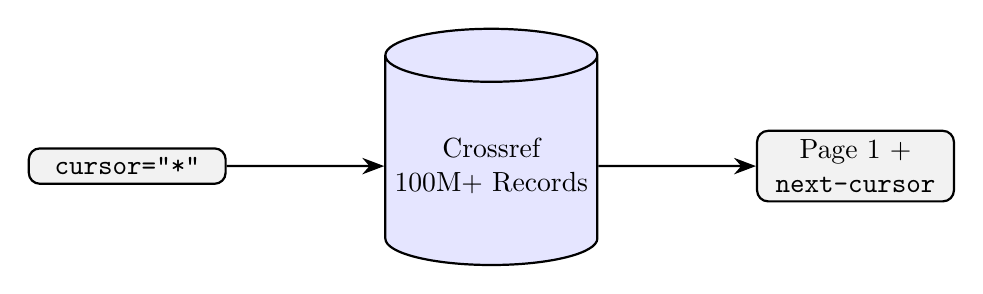
\begin{tikzpicture}[
      node distance=1.5cm and 2cm,
      req/.style={rectangle, draw, thick, rounded corners, minimum width=2.5cm, align=center, fill=black!5},
      db/.style={cylinder, draw, thick, shape border rotate=90, aspect=0.25, minimum height=3cm, minimum width=2cm, align=center, fill=blue!10},
      arrow/.style={-{Stealth[scale=1.2]}, thick}
    ]
    
    \node[req] (r) {\texttt{cursor="*"}};
    \node[db, right=of r] (db) {Crossref\\100M+ Records};
    \node[req, right=of db] (page) {Page 1 + \\\texttt{next-cursor}};
    
    \draw[arrow] (r) -- (db);
    \draw[arrow] (db) -- (page);
  \end{tikzpicture}
  }
  \end{center}
  \vspace{0.2cm}
  Like OpenAlex, Crossref uses cursor pagination, but the cursor strings must be strictly URL-encoded as they frequently contain \texttt{+} and \texttt{=} characters.
\end{frame}

\begin{frame}{Implementation: `issued.date-parts`}
  \begin{block}{The Nested Array Nightmare}
    Crossref stores publication dates as nested arrays: \texttt{[[2023, 5, 12]]} or sometimes just \texttt{[[2023]]}.
  \end{block}
  
  \begin{itemize}
      \item Our \texttt{CrossrefNormalizer} must safely extract the first element of the inner array.
      \item If the month or day is missing, it gracefully falls back to \texttt{None} while preserving the year.
  \end{itemize}
\end{frame}

\begin{frame}{Implementation: The Polite Pool}
  \begin{block}{mailto: Required}
    Similar to OpenAlex, Crossref demands a \texttt{mailto} parameter.
  \end{block}
  
  \begin{itemize}
      \item If omitted, you are routed to the public pool, which is notoriously slow and prone to 503 errors.
      \item Our configuration system automatically injects this into the request session.
  \end{itemize}
\end{frame}

\begin{frame}{Verification}
  \begin{alertblock}{Success Criteria}
    \begin{itemize}
        \item The \texttt{CrossrefProvider} correctly normalizes incomplete date arrays.
        \item Author names are concatenated cleanly (Crossref separates \texttt{given} and \texttt{family} names).
        \item The URL-encoded cursor loop fetches subsequent pages correctly.
    \end{itemize}
  \end{alertblock}
\end{frame}

\end{document}
